\documentclass[10pt,twocolumn,letterpaper]{article}
\usepackage[review]{cvpr}
\usepackage{graphicx,amsmath,amssymb,amsthm,booktabs,array,multirow,xcolor}
\usepackage{microtype}
\definecolor{linkblue}{rgb}{.0,.35,.55}
\usepackage[pagebackref,breaklinks,colorlinks,allcolors=linkblue]{hyperref}
\newtheorem{theorem}{Theorem}
\newtheorem{lemma}{Lemma}
\newtheorem{corollary}{Corollary}
\newtheorem{remark}{Remark}
\newcommand{\R}{\mathbb R}
\newcommand{\E}{\mathbb E}
\newcommand{\Cov}{\operatorname{Cov}}
\newcommand{\cond}{\operatorname{cond}}
\newcommand{\rms}{\operatorname{RMS}}
\newcommand{\DPM}{DPM-Solver++(2S)}
\usepackage[capitalize]{cleveref}
\crefname{theorem}{theorem}{theorems}
\Crefname{theorem}{Theorem}{Theorems}
\hypersetup{pdftitle={When Diffusion Steps Lose Their Inputs: Sharp Injectivity Limits and Inversion Cost},pdfauthor={Anonymous Authors}}

% Expand the row fragment before a booktabs rule begins the next alignment row.
\makeatletter
\newcommand{\tablerows}[1]{\@@input{#1}}
\makeatother

\newcolumntype{Q}[1]{>{\raggedright\arraybackslash}p{#1}}

% Generated by tex_results.py from the verified analysis.
\newcommand{\PrimaryDPMRecovered}{64/64}
\newcommand{\FFHQDPMRecovered}{64/64}
\newcommand{\VEReconstruction}{32/32}
\newcommand{\PrimaryN}{64}
\newcommand{\FFHQN}{64}
\newcommand{\VEN}{32}
\newcommand{\PrimaryCap}{320}
\newcommand{\FFHQCap}{160}
\newcommand{\PrimaryDPMWork}{69.2}
\newcommand{\FFHQDPMWork}{78.2}
\newcommand{\FFHQHeunTwoWork}{158.3}
\newcommand{\FFHQHeunTwoRecovered}{64/64}
\newcommand{\FFHQDPMFlow}{0.0490}
\newcommand{\FFHQHeunTwoFlow}{0.0239}
\newcommand{\PrimaryHeunOneFailure}{46/64}
\newcommand{\PrimaryHeunOneLowResidual}{12}
\newcommand{\PrimaryFailureBound}{5.60\%}
\newcommand{\VEFailureBound}{10.89\%}
\newcommand{\PrimaryContrast}{\ensuremath{-71.9\;[-82.8,\,-60.9]}}
\newcommand{\FFHQContrast}{\ensuremath{-92.2\;[-98.4,\,-85.9]}}
\newcommand{\VEContrast}{\ensuremath{-68.8\;[-84.4,\,-53.1]}}
\newcommand{\PrimaryRefinement}{\ensuremath{3.67\times10^{-5}}}
\newcommand{\VERefinement}{\ensuremath{5.38\times10^{-5}}}
\newcommand{\FFHQRefinement}{\ensuremath{1.94\times10^{-5}}}
\newcommand{\PrecisionFlags}{192}
\newcommand{\TargetMismatch}{\ensuremath{3.37\times10^{-6}}}
\newcommand{\WallOverrun}{0.691}
\newcommand{\HeunFourFlow}{0.0143}
\newcommand{\HeunFourWork}{286.1}
\newcommand{\HeunFourRecovered}{64/64}
\newcommand{\NativeHeunFailure}{7/8}
\newcommand{\NativeHeunWork}{1765}
\newcommand{\NestedRecords}{3,224}

% Generated by analyze_round2.py from verified records.
\newcommand{\FFHQHeunOneRecovered}{5/64}
\newcommand{\PrimarySecantUpper}{\ensuremath{2.73\times10^{-5}}}
\newcommand{\SweepN}{12}
\newcommand{\SweepRows}{144}

\def\confName{CVPR}\def\confYear{2027}
\title{When Diffusion Steps Lose Their Inputs:\\Sharp Injectivity Limits and Inversion Cost}
\author{Anonymous CVPR submission}

\begin{document}
\maketitle
\begin{abstract}
Which diffusion steps preserve enough information to recover their inputs from one saved output?
For a coupled two-stage family with exact Gaussian posterior means of one compact prior, nonnegative prediction weights characterize global smooth invertibility for every dimension, prior and positive source noise.
If either weight is negative, a fixed two-atom prior produces three distinct inputs for the same output at sufficiently small source noise.
Standard sigma-Heun therefore needs a noise ratio of at least $1/2$ at every substep to guarantee inversion universally. The shortest such fixed schedule from $a$ to $0<b<a$ takes $\lceil\log_2(a/b)\rceil$ steps.
On a separately frozen FFHQ64 panel over $2\to1/8$, one-step DPM++2S and two-step Heun each recovered \FFHQDPMRecovered{} clean sources under a \FFHQCap{}-forward Anderson ceiling. DPM++2S used \FFHQDPMWork{} mean iterative forwards with forward RMS \FFHQDPMFlow{} against Heun128, and two-step Heun used \FFHQHeunTwoWork{} with RMS \FFHQHeunTwoFlow{}. One-step Heun recovered \FFHQHeunOneRecovered{}.
\end{abstract}
\section{Introduction}
A single diffusion step can send three distinct image states to the same output. For a coupled family of two-stage steps, we give an exact test for ruling out this loss for every Gaussian posterior denoiser of a compact prior. The two prediction weights must both be nonnegative.

\Cref{fig:collision} illustrates what this test protects. The three source states lie on a line through two images that define an exact posterior denoiser. A coarse Heun step sends all three to the same point. Given the resulting image state, any of the three sources is compatible with the observation, even at zero inversion residual. The log-SNR midpoint DPM-Solver++(2S) step on the same interval sends those sources to three different points. Its output determines which source was used.

The distinction matters when a generative pipeline stores a checkpoint on a trajectory and later needs the preceding state, for instance to replay a stage of an edit. The inverse can know the executed map, endpoints and denoiser and still have only one saved state. Injectivity is the condition for unique recovery under that information contract. A second question is how much work a numerical inverse takes. A third is how closely the forward step follows the intended trajectory.

We study the ordinary discrete step itself. Prior work has solved its residual equation numerically~\cite{hong2024} and shown that an exact one-prediction DDIM step has a unique inverse~\cite{verbii2026}. Here the second prediction consumes a state computed from the first. We show when that coupling admits a global inverse and when it can create multiple roots of the step equation.

\begin{itemize}
\item \textbf{A sharp criterion for two coupled predictions.} Covariance geometry gives a global inverse for nonnegative weights. A fixed two-atom prior gives the converse by making either negative weight dominate at an appropriate input.
\item \textbf{The minimum protected Heun schedule.} The criterion gives a per-step threshold of $1/2$. A collision at the first subthreshold step survives the rest of a fixed schedule, which gives the exact minimum length for universal protection.
\item \textbf{A choice between two successful inverses.} On the separately frozen FFHQ64 panel, both DPM++2S and Heun2 recover all clean sources at the same work ceiling. DPM++2S takes fewer inverse evaluations and Heun2 follows the fine-step trajectory more closely. We measure these properties separately and keep the learned-model comparison distinct from the exact guarantee.
\end{itemize}

\begin{figure*}[t]
\centering
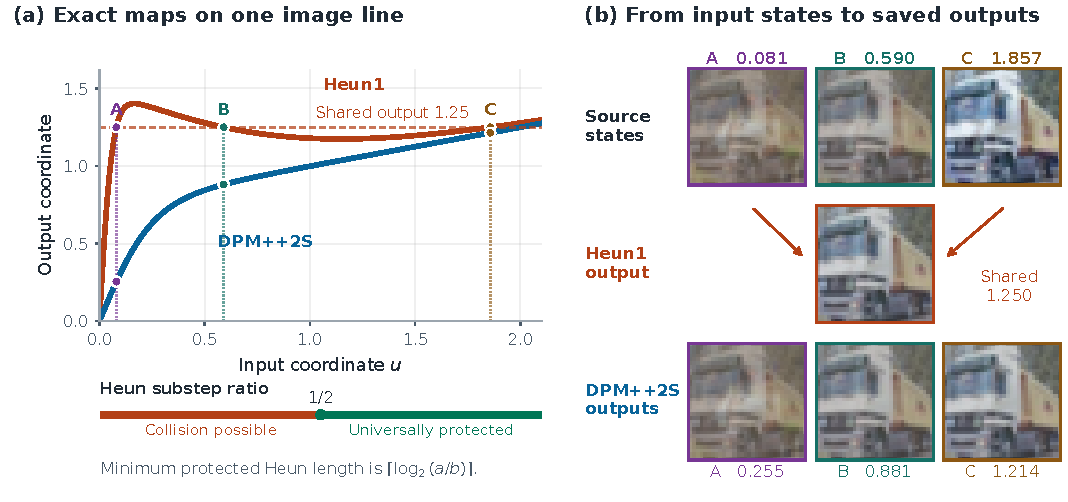
\includegraphics[width=\textwidth]{../figures/figure1.pdf}
\caption{\textbf{One saved Heun output, three compatible inputs.}
\textbf{(a)} The two exact step maps act on the same affine image line $c+uv$ at normalized noise $1\to1/4$. Each of the three marked input brackets contains a root of $H(u)=1.25$, certified by interval arithmetic. DPM++2S separates the same inputs.
\textbf{(b)} The three source tiles are possible reconstructions from the single Heun output. With DPM++2S each source produces a distinct output tile. Below the plot, the ratio rule applies to fixed Heun substeps at positive noise. All tiles use a shared $[-1.8,1.8]$ display mapping because affine states can exceed ordinary image bounds. Displayed coordinates are rounded.}
\label{fig:collision}
\end{figure*}

\section{When the step preserves its input}
\label{sec:theory}
Let $X$ have compactly supported law $\pi$ on $\R^d$ and let $Z\sim\mathcal N(0,I)$ be independent. Write $D_s(x)=\E[X\mid X+sZ=x]$ for the Gaussian posterior mean at $s>0$, using its smooth convolution formula also for atomic priors. Fix $r>0$, $0<q<1$, $\kappa>0$, and real weights with $r+w_1+w_2=1$. At source noise $a>0$ define
\begin{align}
 p_a(x)&=qx+(1-q)D_a(x),\nonumber\\
 F_a(x)&=rx+w_1D_a(x)+w_2D_{\kappa a}(p_a(x)).
 \label{eq:family}
\end{align}
The same prior supplies both posterior means. The first prediction moves the input to the second, even when its own output weight $w_1$ is zero.

\begin{theorem}[Universal invertibility]
\label{thm:sharp}
With these coefficients fixed, $F_a$ is a global orientation-preserving smooth diffeomorphism for every dimension, compact prior and positive source scale $a$ if and only if $w_1,w_2\ge0$. If either weight is negative, the fixed prior $(\delta_{-1}+\delta_{+1})/2$ has an open interval of outputs with at least three preimages each for every sufficiently small $a>0$.
\end{theorem}

\paragraph{Nonnegative weights preserve the input.}
Differentiating the Gaussian posterior mean gives
\begin{equation}
 \nabla D_s(x)=s^{-2}\Cov(X\mid X+sZ=x)\succeq0.
 \label{eq:covariance}
\end{equation}
Thus $D_s$ is a convex gradient~\cite{gribonval2021}, bounded by compactness of the support. Write $A=\nabla D_a(x)$, $B=\nabla D_{\kappa a}(p_a(x))$, and $E=qI+(1-q)A$. The product $BE$ in the step Jacobian $J$ can be nonsymmetric. The positive definite $E$ commutes with $A$, so a similarity transform gives
\begin{equation}
 E^{1/2}JE^{-1/2}
 =rI+w_1A+w_2E^{1/2}BE^{1/2}\succeq rI .
 \label{eq:similarity}
\end{equation}
This gives a local inverse and positive determinant. In Euclidean norm, $\|J^{-1}\|_2\le\sqrt{\operatorname{cond}_2(E)}/r$.

For two inputs, average $\nabla D_a$ along the segment between them and average $\nabla D_{\kappa a}$ along the separate segment between their stage states. Their exact finite difference has the same matrix form as $J$ with these positive semidefinite averages. The matrix is invertible, so distinct inputs have distinct outputs. Since the predictions are bounded, $F_a(x)=rx+O(1)$ is proper. Its image is open by local invertibility and closed by properness, hence it is all of $\R^d$. Supplement~A gives the global inverse bound and a convex-gradient factorization.

\paragraph{A negative weight can fold the map.}
For the two equally weighted atoms, $D_s(x)=\tanh(x/s^2)$. The posterior derivative is steep near its transition at zero and small away from it. If $w_2<0$, evaluating at zero puts both posteriors at their transitions. The product of their derivatives dominates the slope:
\begin{equation}
 \lim_{a\downarrow0}a^4 F'_a(0)=w_2(1-q)/\kappa^2<0.
\end{equation}
If $w_2\ge0$ and $w_1<0$, evaluate at $x=a^2$. The first derivative is $a^{-2}\operatorname{sech}^2(1)$, while the stage stays above $(1-q)\tanh(1)>0$. The second posterior saturates, making its derivative exponentially small. Hence
\begin{equation}
 \lim_{a\downarrow0}a^2 F'_a(a^2)=w_1\operatorname{sech}^2(1)<0.
\end{equation}
The prior stays fixed in both limits. At fixed $a$, the slope tends to $r>0$ in the tails and the outputs go to opposite infinities. Take a short decreasing segment $[u,v]$. Each output strictly between $F_a(v)$ and $F_a(u)$ is attained inside the segment, to its left and to its right. This gives three distinct preimages by continuity.

The necessity is universal over priors and scales. A particular map can remain injective with a negative weight, as for a point-mass prior where the step has constant slope $r$. The converse uses $q<1$. At $q=1$ nonnegative weights still suffice by the symmetric Jacobian. At the coincident-scale boundary $q=1,\kappa=1$ the predictions coincide and the exact criterion becomes $w_1+w_2\ge0$.

\section{What the criterion says about schedules}
\label{sec:solvers}
In additive noise coordinates the probability-flow drift is $f(x,s)=(x-D_s(x))/s$~\cite{karras2022}. Write $\rho=b/a\in(0,1)$ for the denoising ratio. Euler's update is $\rho x+(1-\rho)D_a(x)$, a strongly monotone map with lower slope bound $\rho$ and one denoiser call. The two-evaluation methods in \cref{tab:coeff} have the same residual coefficient $r=\rho$ and differ in how they combine predictions.

For \textbf{sigma-Heun}, the Euler predictor at $b$ is $p_a=\rho x+(1-\rho)D_a(x)$. Substituting it into the trapezoidal update $x+(b-a)[f(x,a)+f(p_a,b)]/2$ produces $w_1$ with the factor $2\rho-1$. The step is universally injective exactly for $\rho\ge1/2$.
For \textbf{explicit sigma-midpoint}, the stage is an Euler step to $(a+b)/2$. Inserting this stage into the midpoint drift gives a negative $w_1$ for every strict denoising ratio.
For \textbf{unthresholded log-SNR midpoint DPM++2S}, the intermediate noise is $\sqrt{ab}$ and the final update uses only the prediction there~\cite{lu2022}. Thus $w_1=0$ and $w_2=1-\rho$. All strict positive denoising ratios satisfy the sign test. Supplement~B derives the three formulas in the same coordinates. When $b=a$, each of these solver steps is the identity.

\begin{table}[t]
\centering\small
\setlength{\tabcolsep}{3.5pt}
\begin{tabular}{@{}lccc@{}}
\toprule
Step & $q=\kappa$ & $w_1$ & $w_2$\\
\midrule
Heun & $\rho$ & $\dfrac{(1-\rho)(2\rho-1)}{2\rho}$ & $\dfrac{1-\rho}{2\rho}$\\[7pt]
Sigma-midpoint & $\dfrac{1+\rho}{2}$ & $-\dfrac{(1-\rho)^2}{1+\rho}$ & $\dfrac{2(1-\rho)}{1+\rho}$\\[7pt]
DPM++2S & $\sqrt{\rho}$ & $0$ & $1-\rho$\\
\bottomrule
\end{tabular}
\caption{Prediction weights in \cref{eq:family}, with $r=\rho=b/a\in(0,1)$. The sign condition applies to the specified ordinary steps with exact posterior means.}
\label{tab:coeff}
\end{table}

\begin{corollary}[Fixed Heun schedules]
\label{cor:schedule}
Fix the ratios $\rho_j\in(0,1]$ of an input-independent denoising schedule. The standard sigma-Heun composition is a global orientation-preserving smooth diffeomorphism for every dimension, common compact prior and positive global scale exactly when every $\rho_j\ge1/2$. For overall $0<b<a$, the minimum length of a schedule with this guarantee is
\begin{equation}
 n_{\min}=\big\lceil\log_2(a/b)\big\rceil.
 \label{eq:nmin}
\end{equation}
\end{corollary}
\begin{proof}
When all ratios meet the threshold, the composition inherits the guarantee. Otherwise use the \emph{first} ratio below $1/2$. With the fixed two-atom prior, reducing the global scale makes that step's source noise small enough to produce a collision. The preceding steps are onto, so two distinct initial states reach the two colliding inputs. Every later deterministic step acts on their equal state and preserves the collision.

The product of $n$ ratios each at least $1/2$ is at least $2^{-n}$. Conversely, $n$ equal ratios $(b/a)^{1/n}$ meet the threshold whenever $n\ge\lceil\log_2(a/b)\rceil$.
\end{proof}

At $2\to1/8$, the grid $2,1,1/2,1/4,1/8$ uses the minimum four Heun substeps and eight denoiser calls. One DPM++2S step has the universal guarantee with two calls. Euler illustrates the separate role of forward fidelity even with a one-call guarantee. The Heun limit is a structural budget for the specified family of schedules. Numerical accuracy and the work of solving for a source must be measured separately.

\section{Related work}
\label{sec:related}
Diffusion and score-based models generate samples by reversing a noising process~\cite{ho2020,songsde2021}. Deterministic samplers integrate the associated probability-flow ODE, either with first-order steps such as DDIM~\cite{songddim2021} or with two-stage and multistep solvers such as Heun's method and DPM-Solver++~\cite{karras2022,lu2022}. Running these samplers backwards is the basis of real-image editing, and the inversion literature has largely treated it as a numerical problem. DDIM inversion approximates each backward step with the forward one~\cite{songddim2021}, and null-text inversion corrects the resulting drift by optimizing the unconditional text embedding~\cite{mokady2023}. A second group solves the implicit equation of each backward step directly. AIDI applies fixed-point iteration with Anderson acceleration~\cite{pan2023aidi}, fixed-point inversion and ReNoise iterate the denoiser at each step to refine the backward state~\cite{meiri2023fpi,garibi2024renoise}, Hong et al.\ invert the executed DPM-Solver discretization exactly up to solver tolerance~\cite{hong2024}, and timestep rescheduling chooses the inversion grid to reduce an error surrogate at a fixed budget~\cite{sun2026}. All of these methods search for a preimage of a step they did not design. Their accuracy is measured by reconstruction, which cannot distinguish the true source from another input with the same output. Whether that preimage is unique is a property of the step itself, and it is the property we characterize. Our experiments use the same Anderson-accelerated fixed-point machinery as AIDI~\cite{walker2011}, so they measure what these solvers can achieve on steps inside and outside the guarantee.

A different line of work changes what is stored rather than how the step is inverted. EDICT, BDIA and BELM couple or extend the sampling recurrence so that it is algebraically reversible from two retained states~\cite{wallace2023,zhang2024,wang2024}. Rex wraps exponential integrators, including DPM++2S as a base scheme, in a reversible coupling~\cite{rex2026}, and near-reversible explicit methods trade a small round-trip error for stability under edits~\cite{barancikova2026}. Edit-friendly DDPM inversion instead stores one auxiliary noise map per step, so that any image is reproduced exactly by construction~\cite{huberman2024ddpm}. These designs obtain exact reversal by retaining extra state, whereas we ask when the ordinary single-output step already has it, and Supplement~I compares the contracts side by side.

Invertibility itself has a longer history. The exact probability-flow ODE defines a diffeomorphism between noise levels, as any well-posed ODE flow does~\cite{songsde2021,chen2018node}, but a finite step need not inherit this property. Invertible residual networks show that a step $x+g(x)$ is a bijection when $\operatorname{Lip}(g)<1$~\cite{behrmann2019iresnet}, a sufficient condition that is far too strong for a large diffusion step whose denoiser Jacobian scales as $R^2/s^2$. Our sufficient condition instead uses the structure of the Bayes denoiser. By Tweedie's formula the posterior mean is the input plus a scaled score~\cite{efron2011tweedie}, so it is the gradient of a convex function with covariance Jacobian~\cite{gribonval2021}, and strongly convex gradients are invertible~\cite{huang2021}. The closest result is Verbii's analysis of the exact one-prediction DDIM step~\cite{verbii2026}, which writes its inverse as a strongly convex program with a unique solution and shows that an amplitude-scaled, off-Bayes score can create multiple roots for a two-atom law. We extend this picture to coupled two-stage steps in the coordinates of the first stage, and our converse is new to that setting. It shows that exact Bayes predictions can themselves collide once one prediction is evaluated at a state produced by the other, and it yields an exact schedule threshold for Heun. Requiring nonnegative combination weights echoes strong-stability-preserving Runge--Kutta methods, which are built from convex combinations of forward Euler steps~\cite{gottlieb2001,gottlieb2018}, although the property preserved here is injectivity rather than a norm bound.

\section{Inverting learned diffusion steps}
\label{sec:experiment}
\begin{figure*}[t]
\centering
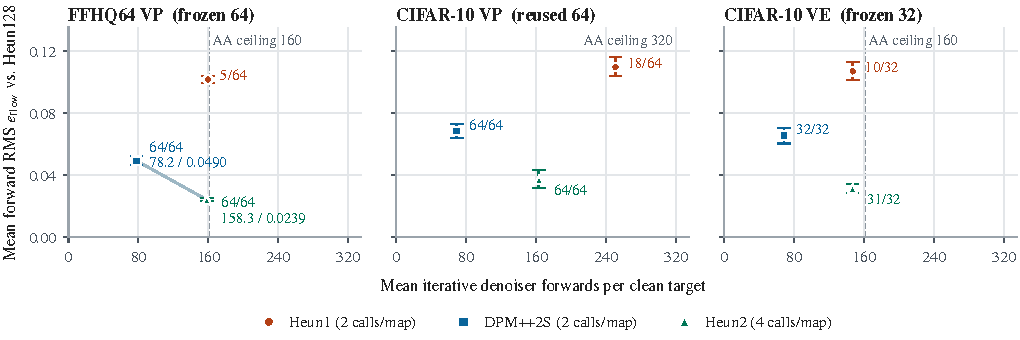
\includegraphics[width=\textwidth]{../figures/tradeoff.pdf}
\caption{\textbf{Two FFHQ64 choices recover the same clean sources.}
DPM++2S uses fewer inverse calls and Heun2 gives lower forward RMS. Marker labels give clean recovery counts. The two linked points also give mean iterative forwards and forward RMS. Bars show 95\% seed-bootstrap intervals for mean forward RMS against Heun128. The panels share axes but use the indicated cohort-specific ceilings. The reused primary panel has saved GPU targets and a CPU inverse. The separately frozen FFHQ64 and VE panels use CPU targets and inverses. \Cref{tab:recovery} includes noisy targets and the other primary maps.}
\label{fig:tradeoff}
\end{figure*}

\begin{table*}[t]
\centering\small
\setlength{\tabcolsep}{7pt}
\begin{tabular}{@{}lrrrrr@{}}
\toprule
Step map & Calls per map & Clean recovered & Noisy recovered & Mean $e_{\rm flow}$ & Mean clean $N_f$\\
\midrule
\multicolumn{6}{@{}l}{\textbf{FFHQ64 VP} \enspace \FFHQN{} separately frozen sources, \FFHQCap{} forwards, CPU targets}\\
\tablerows{generated/ffhq_rows_labeled}
\midrule
\multicolumn{6}{@{}l}{\textbf{CIFAR-10 VP} \enspace \PrimaryN{} reused sources, \PrimaryCap{} forwards, saved GPU targets}\\
\tablerows{generated/primary_rows_labeled}
\midrule
\multicolumn{6}{@{}l}{\textbf{CIFAR-10 VE} \enspace \VEN{} separately frozen sources, \FFHQCap{} forwards, CPU targets}\\
\tablerows{generated/ve_rows_labeled}
\bottomrule
\end{tabular}
\caption{\textbf{Anderson recovery at each cohort's registered ceiling.}
Recovery requires source RMS $e_x\le0.02$. $N_f$ counts iterative denoiser forwards. Each inverse has two initializer calls, with final diagnostics also accounted for separately. The forward reference is Heun128 on the target-generation device. Supplement~E reports source errors, residuals and hybrid work.}
\label{tab:recovery}
\end{table*}

We now treat the denoisers as fixed neural networks. The inverse sees $y=F(x)+\eta$, the operator $F$ and its schedule. It starts at a two-step reverse Euler estimate computed from $y$. Source truth, the seed, intermediate states and the clean version of a noisy target are held by the evaluator. With $\rms(v)=\|v\|_2/\sqrt d$ over the $d$ image coordinates, we measure
\begin{equation}
 \begin{aligned}
 e_x&=\rms(\widehat x-x),& e_y&=\rms(F(\widehat x)-y),\\
 e_{\rm flow}&=\rms(F(x)-F_{\rm ref}(x)).&&
 \end{aligned}
 \label{eq:metrics}
\end{equation}
A recovery has $e_x\le0.02$. The inverse selects by $e_y$, using a residual stopping tolerance of $2\times10^{-6}$. Clean targets have $\eta=0$. Noisy targets use Gaussian noise with coordinate standard deviation $10^{-3}$, paired across maps at each source.

\paragraph{Sources and maps.}
We use the public unconditional EDM CIFAR-10 VP, CIFAR-10 VE and FFHQ64 VP checkpoints~\cite{karras2022,cifar2009,karras2019}. Each source is the state at sigma 2 after Heun64 from sigma 80, initialized with $80$ times a seeded standard Gaussian array. The test interval is $2\to1/8$. We compare two Euler steps, one Heun step, one sigma-midpoint step, one DPM++2S step, and two Heun steps. Two-step grids use EDM's fixed sigma-power schedule with exponent 7. A repeated primary diagnostic also uses the geometric Heun4 grid from \cref{cor:schedule}. The numerical forward reference is Heun128 on the same network and interval. We report its disagreement with Heun64 as a refinement check.

\paragraph{Cohorts and precision.}
The primary \PrimaryN{} CIFAR-VP sources were already observed before the frozen comparison. Their saved targets are from GPU execution and their inverses run on CPU. The fresh \VEN{} CIFAR-VE and \FFHQN{} FFHQ64-VP seeds were frozen separately after disjoint development runs. Their targets and inverses use the same CPU operator. Outer states are float64 and denoisers evaluate in float32. A clean CPU-target replay on the reused primary cohort isolates the effect of the device change. Each inverse runs on one image at a time. The independently seeded source is the unit of analysis. All method, noise and budget comparisons within a cohort are paired by seed.

\paragraph{Inverses and work.}
Anderson acceleration (AA)~\cite{walker2011} extrapolates the target-residual fixed-point map with memory five and damping $0.8$. Two primary controls start from the observed AA iterate available within 80 forwards and continue with L-BFGS~\cite{liu1989} or inexact Newton--GMRES~\cite{saad1986}. The L-BFGS control charges line searches and gradient traversals. Newton--GMRES charges centered finite-difference Jacobian actions, line searches and unfinished work. Primary ceilings are 80, 160 and \PrimaryCap{} iterative denoiser traversals. Each charges forward and backward traversals, including the shared AA warm work for each hybrid. The fresh cohorts use AA with a ceiling of \FFHQCap{} forwards. A forward pass through the \emph{step map} can call the denoiser more than once. We report these calls per map separately from the inverse's actual iterative work, and itemize initialization and final diagnostics in the supplement.

\paragraph{Uncertainty.}
Failure intervals use two-sided exact binomial limits. Mean and paired-difference intervals use 10,000 bootstrap draws of source seeds, with the same resampled indices on both sides of a contrast. Cohorts are summarized separately.

\section{Recovery, forward fidelity and work}
\label{sec:results}

\paragraph{FFHQ64 at 160 inverse forwards.}
On the separately frozen FFHQ64 panel, DPM++2S and Heun2 each recover \FFHQDPMRecovered{} clean sources (\cref{fig:tradeoff,tab:recovery}). DPM++2S uses two calls to advance the state and \FFHQDPMWork{} mean iterative calls to recover it. Heun2 uses four to advance and \FFHQHeunTwoWork{} to recover, with lower mean forward RMS (\FFHQHeunTwoFlow{} versus \FFHQDPMFlow{}). Both also recover all noisy targets at coordinate noise SD $10^{-3}$. Heun1 recovers \FFHQHeunOneRecovered{} clean sources. Its paired clean failure difference against DPM++2S is large (DPM++2S minus Heun1, \FFHQContrast{} percentage points, with a 95\% seed-bootstrap interval).

Both substep ratios of the tested Heun2 grid are below $1/2$ (Supplement~B), placing this successful schedule outside the universal guarantee in \cref{cor:schedule}.

\paragraph{Separate CIFAR-VP and VE protocols.}
DPM++2S recovers \PrimaryDPMRecovered{} clean and all noisy sources on the reused CIFAR-VP panel at \PrimaryCap{} forwards. Euler2 is also successful with similar work, and sigma-midpoint has lower forward RMS with more recovery failures. Heun2 improves forward fidelity and recovers all sources at this ceiling. On the separately frozen CIFAR-VE panel, DPM++2S recovers \VEReconstruction{} under AA\FFHQCap{}. Heun2 recovers 31/32. Zero observed failures give two-sided exact 95\% upper failure limits of \PrimaryFailureBound{} at $N=64$ and \VEFailureBound{} at $N=32$. The Heun64/128 mean RMS disagreements are \FFHQRefinement{} on FFHQ, \PrimaryRefinement{} on CIFAR-VP and \VERefinement{} on CIFAR-VE.

\paragraph{Sensitivity to interval, optimizer and budget.}
On the reused CIFAR-VP seeds, all five maps recovered all 64 sources in both target arms in the earlier, shorter $2\to1/2$ GPU experiment, under a ceiling of 80 \emph{map evaluations}. That cap gives unequal denoiser work across maps. On the long interval, warm-started L-BFGS and Newton--GMRES at the 320-traversal ceiling retain the large Heun1 gap and introduce a few Heun2 misses. A contiguous 20\,s AA allocation including initialization also retains the gap. The native strong-Wolfe L-BFGS diagnostic still has \NativeHeunFailure{} clean Heun1 failures on the first eight reused indices, at a mean of \NativeHeunWork{} charged traversals under an unequal-work protocol. The post-hoc geometric Heun4 repeat meets the half-ratio criterion. At AA320 with CPU targets it recovers \HeunFourRecovered{} clean sources, with forward RMS \HeunFourFlow{} and \HeunFourWork{} mean iterative calls. Supplements~E and F give the complete controls and their budgets.

\paragraph{What the solver comparison identifies.}
At $2\to1/8$, Heun1 uses $(w_1,w_2)=(-6.5625,7.5)$ and evaluates the second prediction at $\sigma=0.125$. DPM++2S uses $(0,0.9375)$ and evaluates it at $\sigma=0.5$. The Heun stage also retains less of the input ($q=1/16$ versus $1/4$). The comparison measures two complete maps under a shared inversion protocol. The coefficient values, cancellation between predictions, stage inputs and second evaluation scale change together. Supplement~G reports the full fixed-stage sweep, which varies the weights while holding the stage fixed.

A small residual can coexist with a large source error. On clean primary Heun1, \PrimaryHeunOneLowResidual{} misses at AA320 fall below the residual stop. For each such pair, with CPU map $F_{\mathrm{CPU}}$ and saved GPU target $y$, the triangle inequality gives
\begin{equation}
 \rms(F_{\mathrm{CPU}}(\widehat x)-F_{\mathrm{CPU}}(x))
 \le e_y+\rms(y-F_{\mathrm{CPU}}(x)).
 \label{eq:secant}
\end{equation}
Dividing this upper bound by $e_x$ gives at most \PrimarySecantUpper{} on those pairs. The pairs exhibit strong compression over finite displacements and are compatible with a poorly conditioned inverse. The CPU-target replay agrees on all \PrecisionFlags{} recovery flags at 160 forwards across the three checked maps. These controls measure recovery and compression at finite precision. The exact multiplicity evidence is the analytic witness in \cref{fig:collision}.

\section{Choosing a step for output-only recovery}
\label{sec:choice}
The sign test changes the choice when unique recovery from one saved state is a requirement across exact priors and scales. At ratio $1/16$, one two-call DPM++2S step meets that requirement. A fixed Heun schedule needs at least four substeps and eight denoiser calls. A checkpoint map $\widehat F$ inherits injectivity if $\operatorname{Lip}(\widehat F-F)<c_*$, where $c_*$ is the exact map's global lower bound on the ratio of output distance to input distance (Supplement~A).

For a learned checkpoint, screen candidates for source recovery on paired calibration states at the intended interval and inverse budget. Compare work among candidates that meet the required recovery rate and forward fidelity. For example, on the FFHQ64 panel in \cref{tab:recovery}, an illustrative mean forward RMS ceiling of $0.03$ against Heun128 admits Heun2 among the maps with complete clean recovery at AA160. At a ceiling of $0.05$, DPM++2S also qualifies and uses fewer calls to advance and recover the state.

\label{mainend}
\clearpage

\section*{LLM Usage Statement}
OpenAI Codex assisted extensively with literature retrieval and synthesis, mathematical derivation and checking, implementation and execution of experiments, figures from equations and saved observations, manuscript drafting and revision, and author-side technical review.
The image tiles come from stored arrays and exact affine constructions.
The authors are responsible for verifying and defending the work.
{\small\bibliographystyle{ieeenat_fullname}\bibliography{references}}
\end{document}
